\documentclass[11pt,]{article}
\usepackage[left=1in,top=1in,right=1in,bottom=1in]{geometry}
\newcommand*{\authorfont}{\fontfamily{phv}\selectfont}
\usepackage[]{mathpazo}


  \usepackage[T1]{fontenc}
  \usepackage[utf8]{inputenc}



\usepackage{abstract}
\renewcommand{\abstractname}{}    % clear the title
\renewcommand{\absnamepos}{empty} % originally center

\renewenvironment{abstract}
 {{%
    \setlength{\leftmargin}{0mm}
    \setlength{\rightmargin}{\leftmargin}%
  }%
  \relax}
 {\endlist}

\makeatletter
\def\@maketitle{%
  \newpage
%  \null
%  \vskip 2em%
%  \begin{center}%
  \let \footnote \thanks
    {\fontsize{18}{20}\selectfont\raggedright  \setlength{\parindent}{0pt} \@title \par}%
}
%\fi
\makeatother




\setcounter{secnumdepth}{0}


\usepackage{graphicx,grffile}
\makeatletter
\def\maxwidth{\ifdim\Gin@nat@width>\linewidth\linewidth\else\Gin@nat@width\fi}
\def\maxheight{\ifdim\Gin@nat@height>\textheight\textheight\else\Gin@nat@height\fi}
\makeatother
% Scale images if necessary, so that they will not overflow the page
% margins by default, and it is still possible to overwrite the defaults
% using explicit options in \includegraphics[width, height, ...]{}
\setkeys{Gin}{width=\maxwidth,height=\maxheight,keepaspectratio}

\title{Legislator Arithmetic: Ideal Points as Neural Networks \thanks{This work is considered preliminary and should not be cited without
permission from the author. The code for this method is available at the
author's github: \url{https://github.com/dargyle/legislator-arithmetic}}  }



\author{\Large Daniel Argyle\vspace{0.05in} \newline\normalsize\emph{FiscalNote}  }


\date{}

\usepackage{titlesec}

\titleformat*{\section}{\normalsize\bfseries}
\titleformat*{\subsection}{\normalsize\itshape}
\titleformat*{\subsubsection}{\normalsize\itshape}
\titleformat*{\paragraph}{\normalsize\itshape}
\titleformat*{\subparagraph}{\normalsize\itshape}


\usepackage{natbib}
\bibliographystyle{apsr}
\usepackage[strings]{underscore} % protect underscores in most circumstances



\newtheorem{hypothesis}{Hypothesis}
\usepackage{setspace}

\makeatletter
\@ifpackageloaded{hyperref}{}{%
\ifxetex
  \PassOptionsToPackage{hyphens}{url}\usepackage[setpagesize=false, % page size defined by xetex
              unicode=false, % unicode breaks when used with xetex
              xetex]{hyperref}
\else
  \PassOptionsToPackage{hyphens}{url}\usepackage[unicode=true]{hyperref}
\fi
}

\@ifpackageloaded{color}{
    \PassOptionsToPackage{usenames,dvipsnames}{color}
}{%
    \usepackage[usenames,dvipsnames]{color}
}
\makeatother
\hypersetup{breaklinks=true,
            bookmarks=true,
            pdfauthor={Daniel Argyle (FiscalNote)},
             pdfkeywords = {ideal point estimation},
            pdftitle={Legislator Arithmetic: Ideal Points as Neural Networks},
            colorlinks=true,
            citecolor=blue,
            urlcolor=blue,
            linkcolor=magenta,
            pdfborder={0 0 0}}
\urlstyle{same}  % don't use monospace font for urls

% set default figure placement to htbp
\makeatletter
\def\fps@figure{htbp}
\makeatother

\onehalfspacing
\usepackage{float}
\floatplacement{figure}{!htb}
\usepackage{booktabs}


% add tightlist ----------
\providecommand{\tightlist}{%
\setlength{\itemsep}{0pt}\setlength{\parskip}{0pt}}

\begin{document}

% \pagenumbering{arabic}% resets `page` counter to 1
%
% \maketitle

{% \usefont{T1}{pnc}{m}{n}
\setlength{\parindent}{0pt}
\thispagestyle{plain}
{\fontsize{18}{20}\selectfont\raggedright
\maketitle  % title \par

}

{
   \vskip 13.5pt\relax \normalsize\fontsize{11}{12}
\textbf{\authorfont Daniel Argyle} \hskip 15pt \emph{\small FiscalNote}

}

}








\begin{abstract}

    \hbox{\vrule height .2pt width 39.14pc}

    \vskip 8.5pt % \small

\noindent We introduce a neural network implementation of ideal point estimation
called NN-NOMINATE that scales well to large datasets and allows
incorporation of additional metadata. We test the model on synthetic
data, the entire corpus of US Congressional votes, and cosponsorship
decisions since the 93rd Congress. These experiments show that the model
behaves as expected and that, when using a held out set of votes as a
validation set, we are able to make informed decisions about the model
structure including the number of dimesions and whether or not to add
covariates.


\vskip 8.5pt \noindent \emph{Keywords}: ideal point estimation \par

    \hbox{\vrule height .2pt width 39.14pc}



\end{abstract}


\vskip 6.5pt


\noindent  \section{Introduction}\label{introduction}

We propose a neural network implementation of ideal-point estimation
that scales well to large datasets and allows incorporation of
additional metadata, which we call NN-NOMINATE. Neural networks are well
suited for ideal point models, and the performance benefit, along with
distributed computing capabilities, allows application of ideal point
estimation to pooled datasets where computation was previously
infeasible due to scale. We demonstrate the algorithm on two different
datasets, the complete history of US Congressional roll call votes and
modern cosponsorship behavior, and compare the results against standard
ideal point estimation techniques.

We demonstrate NN-NOMINATE in two ways. First, we jointly estimate ideal
points over the pooled set of US Congressional roll call votes from
1789-2018. Unidimensional ideal points from the neural network
implementation are similar to the conventional DW-NOMINATE results.
However, cross validation scores indicate that the data are better
explained with more than one dimension. Clustering the multidimensional
ideal points yields intuitive temporal and ideological groupings and
provides a more nuanced picture of ideological polarization.

To evaluate algorithmic performance, we test the resulting estimates on
both training and test data by holding out a subset of legislators'
votes. This allows us to compare the quality of different model
parameterizations and choice of dimensions while still guarding against
overfitting. Specifically, we directly compare the performance of
NN-NOMINATE to different ideal point parameterizations such as
DW-NOMINATE and the conventional Bayesian parameterization.

Second, we take advantage of the fact that many more bills are sponsored
than actually come to a vote and estimate an ideal point distribution
over a large set of sponsorship and cosponsorship decisions in the
93rd-114th Congresses. Cosponsorship provides a different perspective on
legislators' beliefs, independent of strategic voting or administrative
votes of little ideological salience. We treat cosponsorship as a clear
endorsement of a bill's content and assume that a choice not to
cosponsor a bill can be interpreted as something less than full support.
When compared to traditional ideal points, cosponsorship ideal points
show somewhat different trends in polarization and result in a higher
number of optimal dimensions.

\section{Implementing Ideal Points as a Neural
Network}\label{implementing-ideal-points-as-a-neural-network}

This work is inspired by two similar lines of research in political
science and computer science. Speaking broadly\footnote{A complete
  review of the literature in either field is beyond the scope of this
  work, and there are, unsurprisingly, some exceptions to this
  assertion.}, political scientists -- from the the seminal work of
\cite{poole} and \cite{clinton2004statistical}, and up to and including
modern contributions such as \cite{imai2016fast} -- have focused
primarily on ideal point estimation as a means to position legislators
within the ideology space. That these methods also predict votes is
somewhat of an afterthought. On the other hand, computer science
implementations largely focus on using an ideal point framework to
predict legislator votes, without interpreting the ideal points
themselves (for example see \cite{gerrish,kraft}).

Combining the insights of these two fields, we wish to use the
prediction-focused framework of computer science to select the most
accurate model, which in turn would provide the most informative ideal
point estimations for substantive interpretation. We suggest that 1) the
model that predicts the best \emph{on a held out sample of votes}
provides the most insightful ideal points and 2) there is a clear
trade-off between explanatory power and ease of interpretation (for
example in the number of dimensions chosen) in all ideal point models
that should be made explicit.\footnote{We will provide evidence that the
  optimal number of dimensions for ideal point estimation is larger than
  the most common one or two. It is perfectly reasonable to choose to
  rely on two dimensions, but the trade-offs of that choice should be
  clear.}

\subsection{Model Frameworks}\label{model-frameworks}

There are two broad frameworks that have been commonly used for ideal
point estimation. Both tie back to spatial voting theory and the idea
that a legislator will prefer something that is ``near'' to them in the
ideology space. This ideology space can be parameterized with an
aribtrary number of dimensions (denoted with \(K\)), but in most
applications \(K\) is set to be 1 or 2.

The first framework, the NOMINATE family, posits that the probability
that a legislator votes yes on a bill is given by:

\begin{equation}\label{eq:wnom}
prob(vote=yea) = \Phi\left(u_{ijy} - u_{ijn}\right) = \Phi\left(\beta \left[\exp\left(-\frac{1}{2}\sum_{k=1}^s w_k^2 d_{ijyk}^2 \right) - \exp\left({-\frac{1}{2}\sum_{k=1}^s w_k^2 d_{ijnk}^2 }\right)\right]\right)
\end{equation}

\noindent
where \(u_{ijy}\) is the utility legislator \(i\) receives from voting
yes (\(y\)) on proposal \(j\).\footnote{For simplicity, we are
  surpressing the time dimension that is often present in these models.
  However, NN-NOMINATE generalizes to include dynamic ideal points as is
  discussed later in the paper. See also \cite{carroll2009measuring} for
  more detail about the background of this model.} This utility is
expressed in terms of the squared distance \(d_{ijyk}^2\) between a
legislator's ideal point and the ``yes'' outcome point (and similarly
\(d_{ijnk}^2\) is the distance between the legislator's ideal point and
the ``no'' outcome point). There are also a set of salience weights
\(w_k^2\) which allow different dimensions to have more impact on the
final voting decision. The function \(\Phi\) is commonly a normal or
logistic cdf, which makes this model essentially a probit or logit
regression over a quantity determined by the ideal points and bill
attributes. The parameter \(\beta\) represents the signal to noise ratio
\citep{wnominate}. A high value corresponds to votes being largely
deterministic, a lower value suggests more randomness. For convenience,
we will denote the inner portion of this equation as

\begin{equation}\label{eq:jointwnom}
NOM = \exp\left(-\frac{1}{2}\sum_{k=1}^s w_k^2 d_{ijyk}^2 \right) - \exp\left({-\frac{1}{2}\sum_{k=1}^s w_k^2 d_{ijnk}^2 }\right)
\end{equation}

\noindent
as it is will be estimated in its own layer in the neural network.

The second framework, the item-response family, commonly associated with
\cite{clinton2004statistical}, predicts a vote as follows:

\begin{equation}\label{eq:irt}
prob(vote=yea) = \Phi\left(\beta_j \cdot \mathbf{x}_i + \alpha_j\right)
\end{equation}

\noindent
where \(\mathbf{x}_i\) is a \(K\) dimensional vector of ideal points and
\(\Phi\) can correspond to either a logistic or probit model. The bill
level parameter \(\beta_j\), sometimes refered to as polarity, is
multiplied with the ideal point vector and determines the lean of the
bill. The parameter \(\alpha_j\), sometimes referred to as popularity,
determines a baseline approval rate for a specific proposal.

\subsection{The Neural Network}\label{the-neural-network}

While neural networks have become strongly associated with deep learning
and black box prediction generation, they are, in essence, flexible
optimization systems fitted using various forms of gradient decent
algorithms.\footnote{Indeed, while not directly applicable to the models
  contained here, there are several papers proving that feed forward
  neural networks can approximate any continuous function
  \citep{cybenko1989approximation, hornik1991}} All that is required to
estimate an ideal point model using a neural network is to set the
network structure to match the underlying framework of the ideal point
model. One example can be seen in Figure \ref{fig:model1}, which
represents the architecture of a W-NOMINATE model. We will walk through
each layer of this example in some detail as a baseline for further
exploration.

\begin{figure}

{\centering 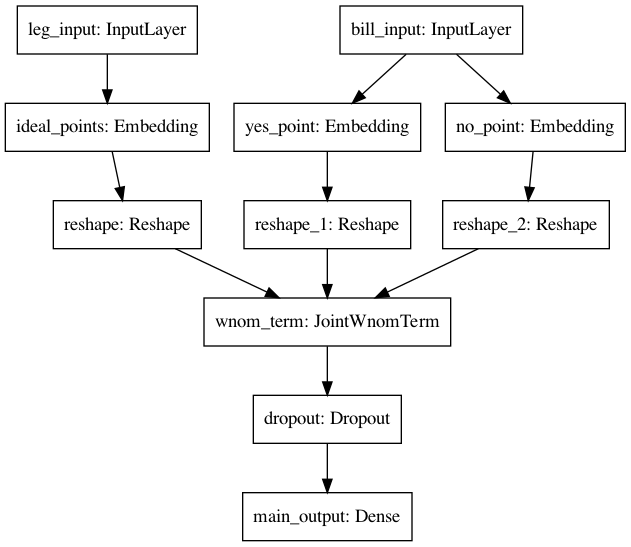
\includegraphics[width=0.75\linewidth]{model}

}

\caption{\label{fig:model1}Base Model}\label{fig:unnamed-chunk-3}
\end{figure}

\begin{itemize}
\item
  Input layers: The inputs to this model consist of numeric identifiers
  for both legisators and bills.
\item
  Embedding layers: These layers take the numeric identifiers and
  convert them into continuous parameters, for example mapping a
  specific legislator to her ideal point vector. In this model there is
  one ideal point embedding for legislators, and two embeddings for
  bills, the yes point and the no point, that correspond to numeric
  values associated with W-NOMINATE style estimation. The ideal point
  layer is restricted in two ways to make the results match more closely
  to the W-NOMINATE framework. First, the model includes orthogonality
  regularization on the ideal points \citep{orthreg1, orthreg2}. This
  penalizes correlation between ideal point dimensions and ensures that
  the resulting estimates are orthogonal so that each dimension
  represents a unique facet of ideology, rather than a slight variant of
  the same overall single dimension. Ideal point embeddings are also
  given a maximum norm constraint, which ensures that the norm of the
  ideal point vector for any legislator lies within the unit hypersphere
  (a common feature of W-NOMINATE).\footnote{Note that the maximum norm
    constraint does not require that any legislator actually attain a
    unit norm. This differs somewhat from existing implementations which
    seem to ensure all dimensions fill the range from {[}-1, 1{]}. If
    this behavior is desired, it can be easily fixed in postprocessing.}
\end{itemize}

\begin{itemize}
\item
  Reshape layers: Because they are often used for text analysis, by
  default embedding layers assume that there is a sequence of ids to to
  transform into the embedding space. Since we have only a single id to
  embed, these layers drop the dimension associated with the sequence to
  form a two dimensional tensor.
\item
  JointWnomTerm layer: The embedded and reshaped data is fed into a
  custom neural network layer that implements the calculation in
  \ref{eq:jointwnom}. This includes combining the ideal points, the yes
  points, the no points, as well as calculating the salience weights
  \(w_k\) for each layer.
\item
  Dropout layer: Dropout regularization, as proposed by \cite{dropout},
  has become an extremely common way of limiting model overfitting,
  often with the additional benefit of improved behavior during model
  training. Dropout layers set a proportion of model weights to 0 at
  random during iterations of the training process. This prevents any
  single weight dominating the prediction of the algorithm. In this
  specific instance, the dropout layer operates over the salience
  weights and sets the weights for any given ideology dimension to 0 for
  a specific iteration of the optimzation algorithm, relying only upon
  the other dimensions to make a vote prediction. In practice, this has
  resulted in better model performance in terms of observable metrics
  and by limiting overfitting during the training process.
\item
  Dense layer: The quantity obtained in the JointWnomTerm layer is then
  used as an input to a Dense layer, parameterised as a logistic
  regression (i.e.~sigmoid activation and binary\_crossentropy loss).
  This returns an estimate for \(\beta\) as well as generating the final
  prediction.
\end{itemize}

The data is given as a batch of triples,
\((legislator\_id, bill\_id, vote)\). The identifiers are fed into the
input layers and subsequently into the embeddings to generate the
predictive parameters of the network. The vote itself is used as the
outcome value of the final model layer (the logistic parameterized Dense
layer).

\section{Testing the Neural Network
Implementation}\label{testing-the-neural-network-implementation}

We demonstrate that the neural network implementation works at least as
well as existing methods through two simple tests. The first is to test
the model on synthetic data, generated with known parameters, and
determine how well the method recovers these known values. The second is
to check that the results match the commonly used implementations of
W-NOMINATE \citep{wnominate} and item response \citep{pscl} ideal
points.

\subsection{Recovering Known Ideal
Points}\label{recovering-known-ideal-points}

The synthetic data is generated to have 3 known dimensions, where the
random predictions are generated in the NOMINATE parameterization found
in equation \ref{eq:wnom}. To guard against overfitting to specific
synthetic votes, we train the model on a subset of the data and test it
on 20\% of the synthetic votes as a held out set. This means that a
legislator's ideal point is determined only by the votes in the training
sample and that a bill's parameters are determined only by the subset of
votes on that bill that appear in training. An additional implication of
this is that at least some votes on a bill must appear in the training
set for the bill to appear in the test set.

There are two primary benefits to using a held out sample. First,
relying on an out of sample evaluation set is often used to determine
when a neural network has converged while estimating a model. There is
little point in continuing to optimize a model where out of sample
performance has plateaued and doing so usually results in overfitting.

Second, performance on a held out sample can be used to make additional
decisions about the model structure, including parameterization choices
or for evaluating distributional assumptions.\footnote{A recent paper by
  \cite{marble2017much} uses a held out set to discuss the predictive
  power of ideal points in survey data, and in doing so estimate ideal
  points on Senate votes from the 111th-114th congress using a heldout
  set and cross-validation. To our knowledge, there have not been other
  attempts to use this out of sample validation strategy more broadly.}
For example, how does making the ideal points dynamic affect the model
performance? What is the optimal number of ideal point dimensions? An
additional dimension may offer an improvement in out of sample
prediction, but it almost always increases in sample performance. An out
of sample performance test provides an objective metric to determine the
optimal number of dimensions to include.\footnote{It is not as simple as
  saying that ``the model that fits best on test data'' is the right
  answer. In some cases it is preferable to say that this is the first
  model that attains a near minimum.} If a practitioner finds it
undesirable to omit votes in this fashion, the model could then be refit
on the entire dataset using the model setup that performed best on the
test data.

\begin{figure}

{\centering 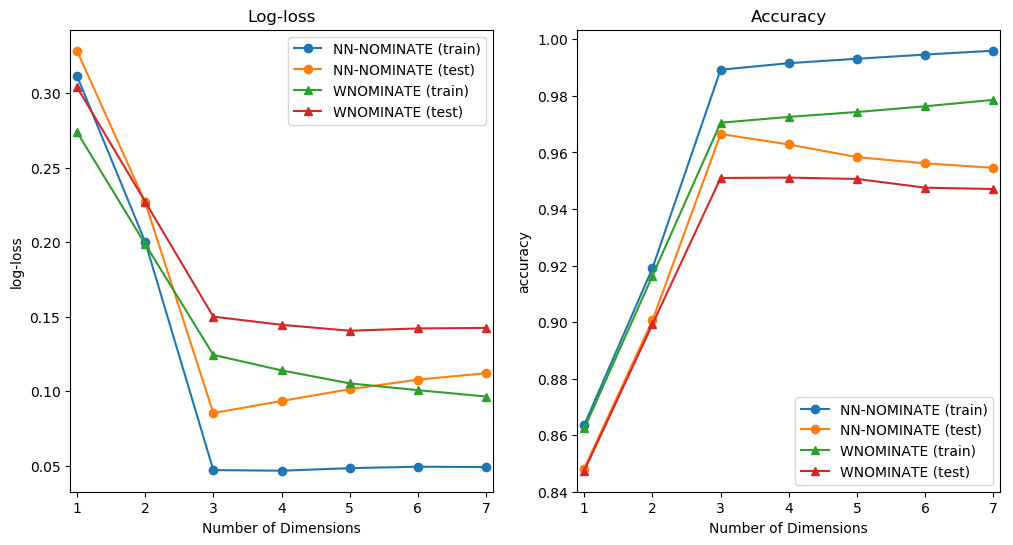
\includegraphics[width=1\linewidth]{test_metrics_with_wnom}

}

\caption{\label{fig:testmetricswnom}Performance metrics on Synthetic Data with W-NOMINATE}\label{fig:unnamed-chunk-4}
\end{figure}

Figure \ref{fig:testmetricswnom} shows the model performance of
NN-NOMINATE on synthetic data, varying the number of dimensions in the
model. For comparison, we also include the same quantities for
W-NOMINATE, obtained using the wnominate package in R. We evaluate two
metrics, accuracy (whether or not the vote was predicted correctly) and
log-loss (a common metric used in classification problems). Log-loss is
useful because it provides an idea of how good the probability estimates
of a model are, and penalizes over-confident predictions. We see that
the log-loss decreases rapidly and is minimized at the optimal number of
dimensions on the test data, following which the test log-loss begins to
increase. Training accuracy shows similar patterns, attaining best
performance on the known optimal number of dimensions. NN-NOMINATE and
W-NOMINATE shows the same mechanics over training and test data. It
appears that for the synthetic dataset at least, NN-NOMINATE (slightly)
outperforms the commonly used WNOMINATE package attaining lower log loss
and higher accuracy on this specific test data.

\begin{table}

\caption{\label{tab:unnamed-chunk-6}\label{tab:corr}Correlations between known and estimated ideal points}
\centering
\begin{tabular}[t]{lrrr}
\toprule
  & true\_coord1D & true\_coord2D & true\_coord3D\\
\midrule
coord1D\_nn & 0.998 & -0.060 & -0.038\\
coord2D\_nn & -0.031 & -0.766 & 0.703\\
coord3D\_nn & 0.010 & -0.635 & -0.708\\
coord1D\_wnom & -0.992 & 0.064 & 0.032\\
coord2D\_wnom & 0.002 & 0.756 & -0.673\\
coord3D\_wnom & -0.008 & -0.598 & -0.708\\
\bottomrule
\end{tabular}
\end{table}

Additionally, Table \ref{tab:corr} shows correlations between the known
ideal points (true\_coord1D), estimates from NN-NOMINATE (coord1D\_nn),
and estimates from W-NOMINATE (coord1D\_wnom. The correlation between
the first dimension of the true and estimated ideal points is near
perfect near perfect across both methods. The correlations in the other
dimensions are somewhat smaller, although given that the synthetic data
was generated with the first dimension having a higher salience weight
than the other two this is understandable. Also, because the model was
only fit on 80\% of the data in training, some imprecision is expected.
An equivalent chart on the full dataset yields stronger correlations
across all dimensions.

\subsection{Comparisons on real data}\label{comparisons-on-real-data}

\begin{figure}

{\centering 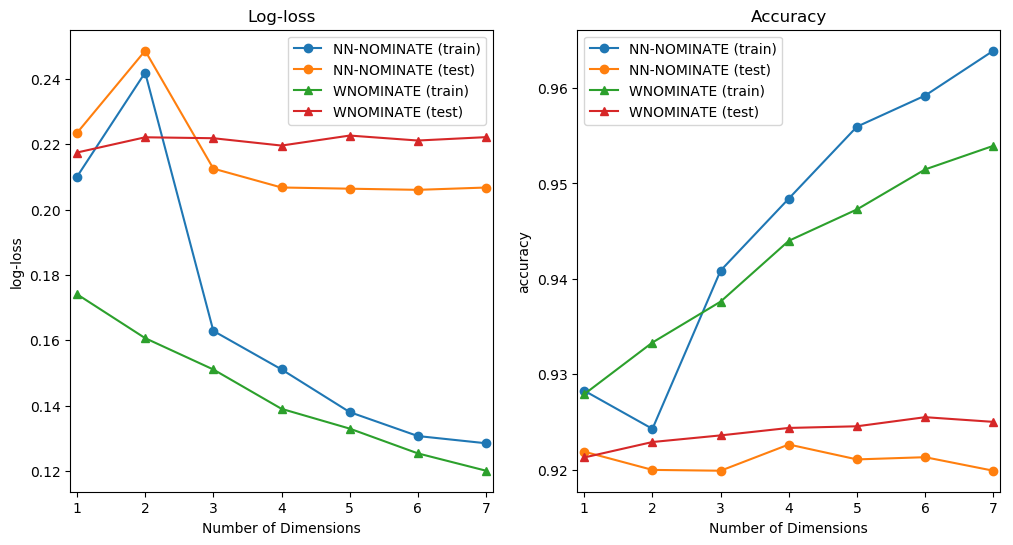
\includegraphics[width=1\linewidth]{votes_metrics_with_wnom}

}

\caption{\label{fig:votesmetrics}Model metrics on 110th-115th Senate}\label{fig:unnamed-chunk-7}
\end{figure}

In Figure \ref{fig:votesmetrics}, we show the same model evaluation
metrics on real world data from the 110th-115th US Senate, which is
roughly the same size as the synthetic test set. In this case there
seems to be little evidence that there exists more than one dimension in
the test data, as both NN-NOMINATE and WNOMINATE improve very little, if
at all, by adding additional dimensions.

\begin{figure}

{\centering 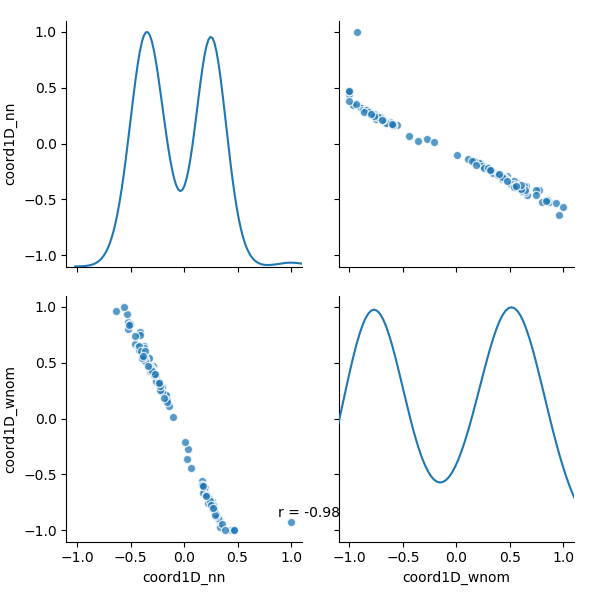
\includegraphics[width=0.75\linewidth]{votes_comp_plot}

}

\caption{\label{fig:votescompplot}NN-NOMINATE and WNOMINATE estimates comparison on 110th-115th Senates}\label{fig:unnamed-chunk-8}
\end{figure}

We can also use simple correlations between the estimated ideal points
to make sure that the ideal point space is similar across estimation
methods. The unidimensional results are shown in Figure
\ref{fig:votescompplot}, which includes the distribution of the ideal
points on the diagonal and a scatter plot with correlation on the
off-diagonal.\footnote{The apparent cause of this is the orthogonality
  regularization and/or the maximum norm constraint which seem to behave
  oddly when imposed in a single dimension. A fix for this problem is
  forthcoming.} The results are nearly identical, with strong
correlations between the two estimation procedures, although there is
one outlier in the NN-NOMINATE results. Note that since ideal points are
not independently identified, including up to dimension switching and
other problems, these results do not match in sign.\footnote{Indeed
  labels often switch across runs of the same model. The exception is
  for NN-NOMINATE, which because of initialization choices (we impose
  initial values for Republicans in the sample on ther right and
  Democrats on the left), almost always results in the first dimension
  being the dimension most strongly related to party. Note that the
  predictive results do not depend on this initialization choice, and
  that it is merely selected for convenience.} Additionally, it is often
the case that NN-NOMINATE results in ideal points that are smaller in
maginitude on average than the WNOMINATE package.

\section{Results and applications}\label{results-and-applications}

While it is comforting to know that a new implementation of an existing
model returns similar results, NN-NOMINATE is capable of more than the
existing implementations. The first is large scale ideal point
estimation, for example fitting models on the entire history of the US
Congress locally on a laptop. The second is to demonstrate the
extensibility of the framework, where the model can be extended very
simply to include covariates as well as more complicated representations
of a bill than existing representations.

\subsection{Large scale
implementation}\label{large-scale-implementation}

We examine two large datasets, all of which can be fitted easily on most
common computers.\footnote{Neural networks have a reputation as require
  lots of processing power, including the use of graphics cards.
  However, for a straightforward model like this, such processing power
  is not necessary. Formal performance comparisions to existing methods
  is forthcoming. } The first is simply the entire history of US
rollcalls. Additionally, this model is dynamic, making it similar to the
DW-NOMINATE parameterization. A legislators ideal point at time \(t\) is
decomposed into a linear function of time,
\(x_{ikt} = x_{ik} + \delta_{ik} t_i\), where \(x_{ik}\) is a constant
ideal point for legislator \(i\) in dimension \(k\), \(\delta_{ik}\) is
a drift parameter for legislator \(i\) on dimension \(k\), and \(t_i\)
represents how long a legislator has been serving in congress.\footnote{A
  full exposition of the math math behind the dynamic part of
  DW-NOMINATE is available in \cite{carroll2009measuring}. NN-NOMINATE
  is capable of estimating any polynomial function of time, but a linear
  parameterization matches the traditional DW-NOMINATE choice and adding
  additional time dimensions make little different to the results. Note
  that NN-NOMINATE, unlike DW-NOMINATE, does not impose any
  orthogonality conditions on the polynomials themselves. A diagram of
  the dynaic NN-NOMINATE is available in \ref{fig:modeldynamic} in the
  appendix.}

\begin{figure}

{\centering 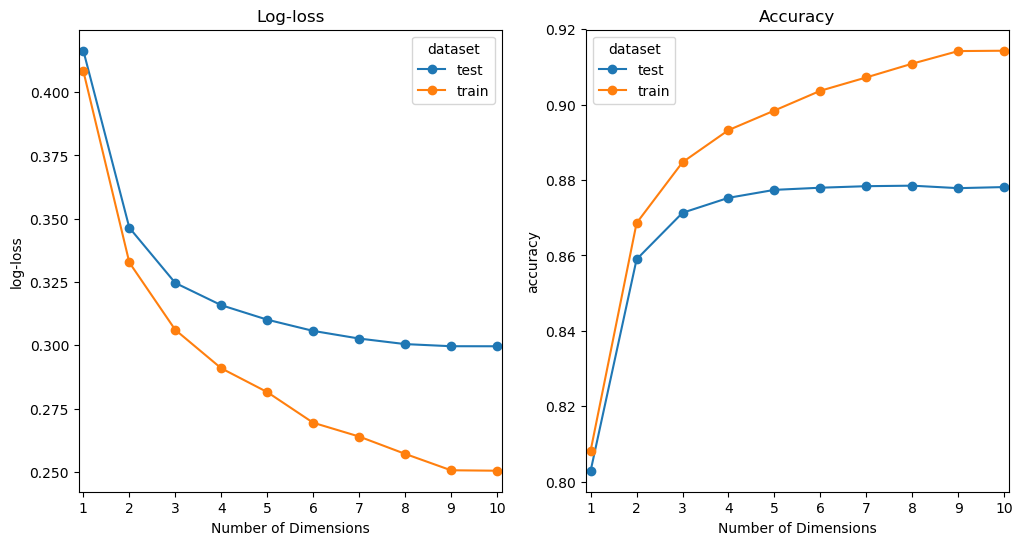
\includegraphics[width=1\linewidth]{full_votes_metrics}

}

\caption{\label{fig:fullvotesmetrics}Metrics on Ideal-Points from the 1st-115th Congresses}\label{fig:unnamed-chunk-9}
\end{figure}

A similar dimension tradeoff calculation to the above test cases is
shown in Figure \ref{fig:fullvotesmetrics}. This shows that over the
entire dataset log-loss on the test data decreases until there are at
least 8 dimensions; however, the incremental improvement for the last
few dimensions is small and does not have a large impact on the accuracy
score. There is some evidence that there are more dimensions to
conventional 1 or 2 dimensional model as there is a non-negligible
improvement to adding the 3rd and 4th dimension.

The second dataset is the set of all cosponsorship decisions from the
93rd-114th US Congresses. This idea goes back at least to
\cite{talbert2002setting}\footnote{See also \cite{aleman2009comparing}.},
who find that there are more dimensions in cosponsorship decisions than
in voting. Since so many voting decisions include strategic concerns,
cosponsorhip, a potentially less impactful choice, could allow
legislators to espouse a wider variety of policy opinions (and thus
require additional dimensions in the modeling process).

In this case, a ``yes'' vote is considered to be sponsoring or
cosponsoring a bill, whereas everyone who did not is assumed (at least
by opportunity cost) to be a ``no''. Note that this data is much noiser
than votes. Since so many bills are introduced that do not proceed in a
given session, there are likely many cases where a legislator would have
preferred that a bill pass even if they did not have the opportunity to
copsonsor it. Because of this, we add additional dropout layers on the
bill parameters themselves. This limits the extent to which the model
can overfit to noise in the dataset. The results in
\ref{fig:fullcosponsorsmetrics} show that there is again some benefit to
including additional dimensions beyond the conventional 1 or 2. However,
the incremental effect of each individual dimension is rather small
beyond 4-5. Examining voting data for the same period (available in
\ref{fig:93votesmetrics} in the appendix) shows no clear indication that
there are any more dimensions in cosponsorship than in voting.

\begin{figure}

{\centering 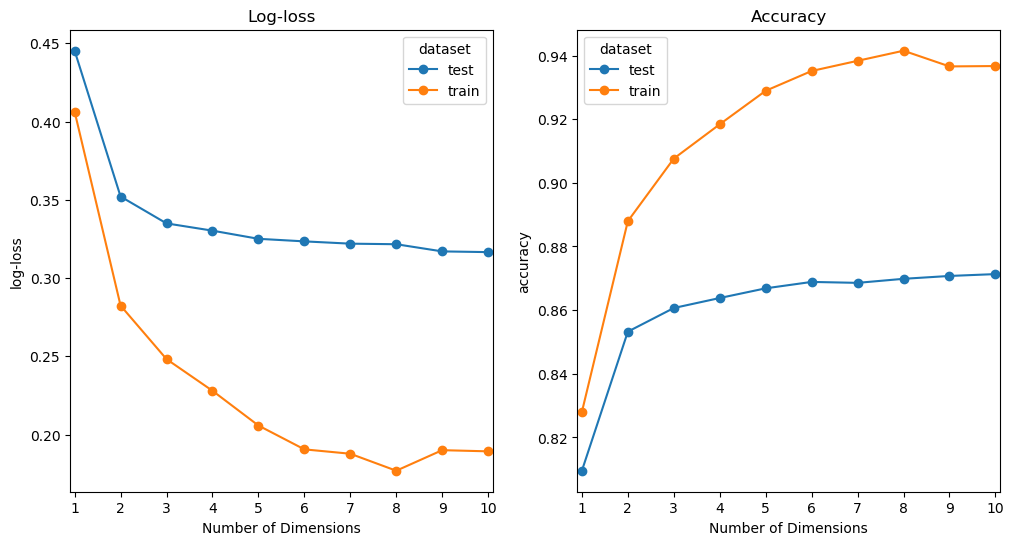
\includegraphics[width=1\linewidth]{full_cosponsor_metrics}

}

\caption{\label{fig:fullcosponsorsmetrics}Metrics on Cosponsorship 93rd-115th Congresses}\label{fig:unnamed-chunk-10}
\end{figure}

While the above results could be construed as evidence, that there are
fewer dimensions in cosponsoring decisions than there are in voting it
seems equally plausible, that the model is more easily fitting to noise
in the cosponsorship decisions so rapidly that the true policy
preference dimensions.

\subsection{Including covariates}\label{including-covariates}

We also extend the model to include covariates. As an example, it is
plausible that a legislator might behave differently while in the party
that controls the chamber. One way this might be observerd is that a
legislator in the party in power is more likely to vote yes, on average,
than someone in the minority party. This could even be the case when the
match with their ideal point is very close, but due to party pressure a
legislator could deviate from this to some extent. As such we estimate
the models from the previous section including a variable indicating
that a legislator is in the party in power so that the logistic layer
now becomes:

\begin{equation}
prob(vote=yea) = \Phi\left(\beta \left[\exp\left(-\frac{1}{2}\sum_{k=1}^s w_k^2 d_{iyk}^2 \right) - \exp\left({-\frac{1}{2}\sum_{k=1}^s w_k^2 d_{ink}^2 }\right)\right] + \gamma * pip_{ik}\right)
\end{equation}

\noindent
where \(\gamma\) represents the effect of being in the party in
power.\footnote{Extending the neural network in this way is relatively
  straightforward. Prior to the final dense layer, the JointWnomLayer
  output is concatenated with an additional input layer which becomes
  another explanatory variable in the final logistic regression layer. A
  version of this is shown in the appendix, Table
  \ref{tab:modelcovariates}} The results show that this factor is
positive, as expected, but that the magnitude represents only a very
small difference in vote probability. Note that the NN-Nominate
framework does not easily lend itself to hypothesis testing. One way to
achieve this would be a parametric bootstrap (ala Poole and Rosenthal)
but this has not been attempted.\footnote{One intriguing path forward is
  suggested by \cite{mandt2017stochastic} who show that under certain
  conditions stochastic gradient decent (as is used in neural networks)
  can proxy for Bayesian inference.}

Additionally, while a discussion of using a text representation of a
bill, rather than a simple indicator value, is beyond the scope of this
work this is a prime area of current research (for example see
\cite{kornilova2018party}). These models work by building embedding
representations of the bills themselves and then determining legislators
ideal points relative to this more robust representation of a bill.
While the accuracy of these models does not yet match that of the bill
indicator approach, these models have the strong advantage of allowing
out of sample prediction on new bill text. This means that we can
determine how a legislator would vote on new bills, as they are
introduced (for more we refer you to the \cite{kornilova2018party}).

\section{Conclusion}\label{conclusion}

We have shown that ideal point estimation is a natural fit for a neural
networks and that we can replicate existing parameterizations using this
new system. However, we feel that this is only scratching the surface of
their potential. We believe that extending this framework, both with
ideas mentioned above and others, will yield new and important insights
into the legislative process.

\hypertarget{refs}{}

\clearpage

\section{Appendix}\label{appendix}

\appendix

\begin{figure}

{\centering 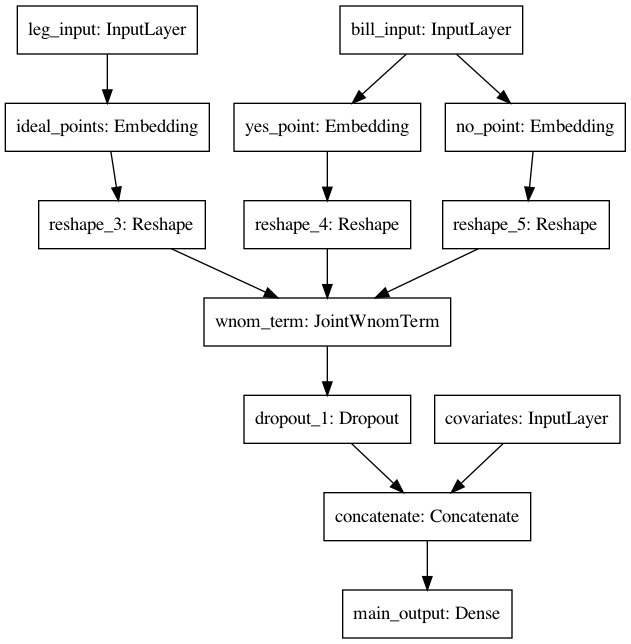
\includegraphics[width=0.75\linewidth]{model_covariates}

}

\caption{\label{fig:modelcovariates}Base Model Including Covariates}\label{fig:unnamed-chunk-11}
\end{figure}

\begin{figure}

{\centering 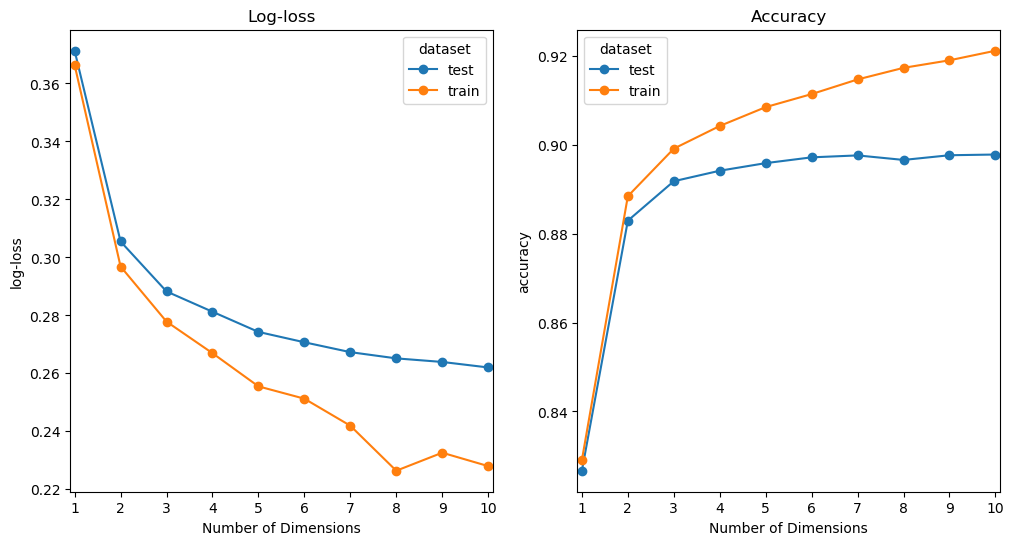
\includegraphics[width=1\linewidth]{93_votes_metrics}

}

\caption{\label{fig:93votesmetrics}Metrics on Ideal-Points from the 93rd-115th Congresses}\label{fig:unnamed-chunk-12}
\end{figure}

\begin{figure}

{\centering 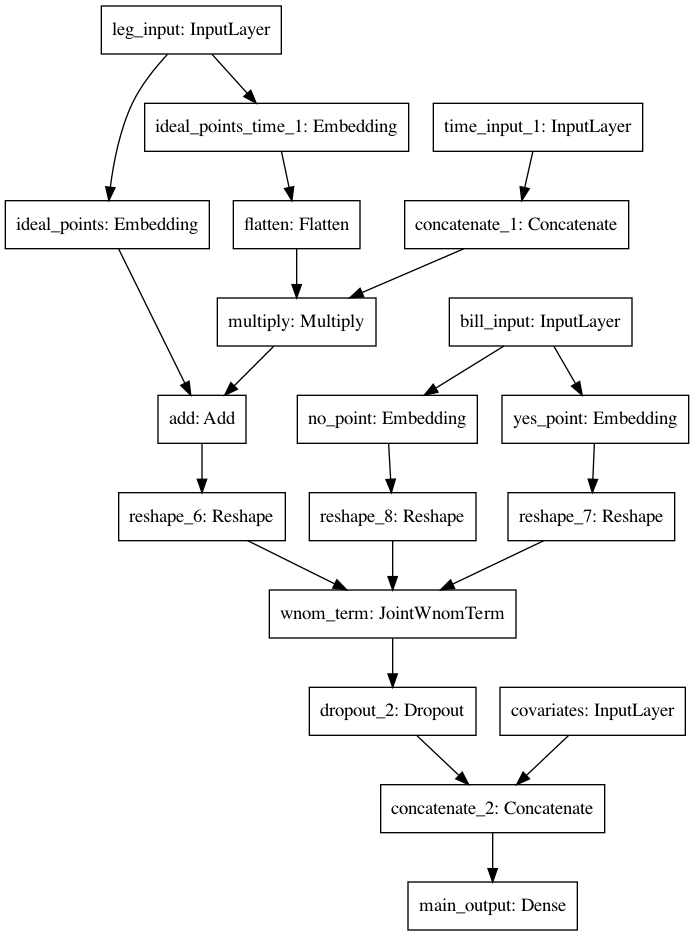
\includegraphics[width=0.75\linewidth]{model_dynamic}

}

\caption{\label{fig:modeldynamic}Base Model Including Dynamic Components}\label{fig:unnamed-chunk-13}
\end{figure}

\clearpage




\newpage
\singlespacing
\bibliography{nnnominate.bib}

\end{document}
